\subsection{The UNIX shell}
\label{bash}
Much can be said about the The UNIX time sharing system
\cite{unix78}, \cite{unixdesign}. It was developed in the early
1970's by Dennis Ritchie and Ken Thompson and featured many
new concepts and abstractions which are still widely used today,
like the file system and its naming and file descriptor concepts,
inter-process communication mechanisms and the command line interface
often referred to as ``the Shell'' \cite{unix78}.

It was also written in a new programming language developed by
Ritchie and Brian Kernighan, called the \textit{C} programming
language \cite{c}. So it delivered exactly what today is missing
in the distributed systems community: a complete stack.

\begin{figure}[h]
  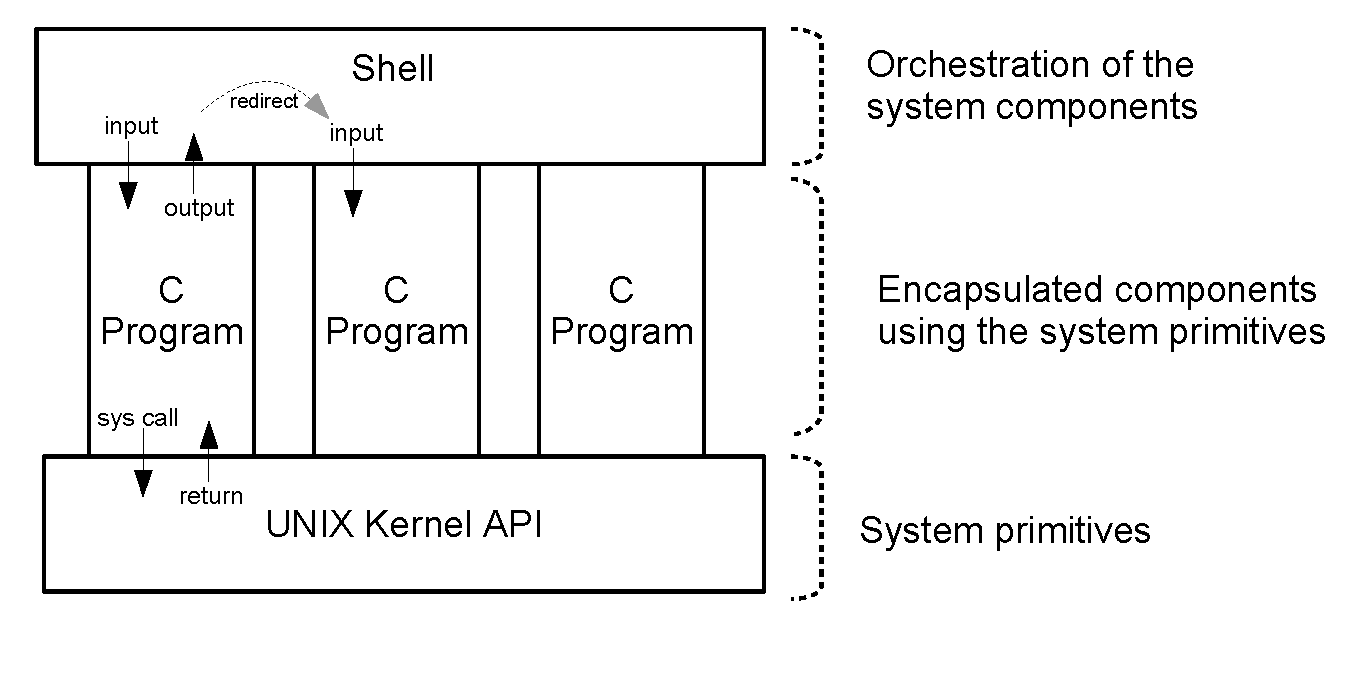
\includegraphics[scale=0.6, keepaspectratio]{unixstack.pdf}
  \caption{Conceptional stack of the original UNIX system}
  \label{unixstack}
\end{figure}

As shown in Fig.\ref{unixstack} the operating system and its
kernel API are positioned at the bottom of the stack. Representing the
foundation by providing basic system primitives in terms of
storage and persistence (memory, file system) but also in terms of
communication (file descriptors, sockets, pipes) although it can be
said that all of these concepts are unified behind an universal channel
concept, namely the file descriptor. Hence the proverb ``In UNIX,
everything is a file''.

The system components are instances of the concept of a \textit{process}.
Encapsulated units of program instances, using virtualized resources like
CPU and memory without any knowledge about other processes and requesting
the system's primitives and services via so called \textit{system calls}.

On top of the stack lies the shell, interfacing with the user.
Using a different language than the system components, its purpose is
to allow the user to control and orchestrate the system by starting
programs (creating a new system component by initiating a new process)
and by either persisting the output of the program to the file system or
chaining subsequent program calls, redirecting the output of one
program to be the input of the next program in the chain
(\textit{pipe mechanism}). Although it is possible for processes
to communicate with other processes indirectly via inter-process communication
mechanisms like \textit{named pipes} or \textit{sockets}, the default
mode of operation is that each process receives its input data from
a designated input channel called \textit{standard in} (stdin) and
can choose between two designated output channels, named
\textit{standard out} (stdout) and \textit{standard error} (stderr),
which direct the output back to the shell who created the process.

This means that each component doesn't know and doesn't have to know
how the whole composition, of which it is being part of.
It only knows where its inputs come from and where to produce its
output to. In my opinion, this bears much resemblance to the basic
notion of a function and function composition in functional programming.
Also the notion of autonomous processes seem very similar to what
is today known as \textit{Actors} in the \textit{Actor Model},
as introduced in chapter \ref{actorModel}.

\begin{wrapfigure}{l}{0.5\textwidth}

  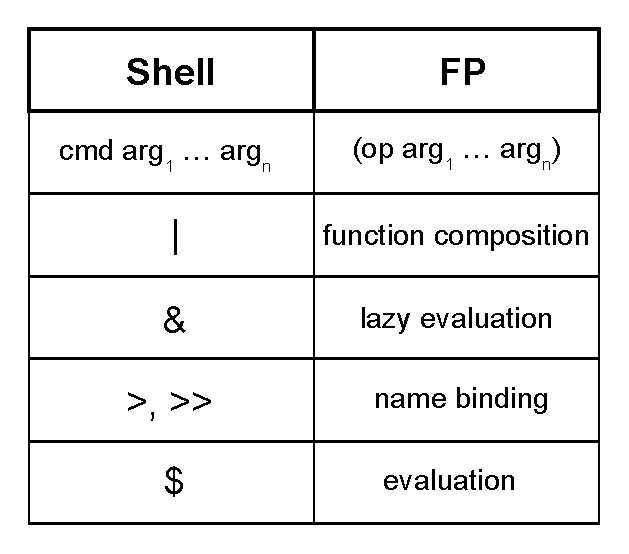
\includegraphics[width=0.5\textwidth]{bash.pdf}
  \caption{Mapping of concepts from the original UNIX shell to
          functional programming concepts.}
  \label{bashmapping}

\end{wrapfigure}

In fact many of the core features and language constructs of a modern
UNIX shell like the \textit{Bourne Again Shell} (bash) \cite{bash}
can be mapped to concepts used in languages following the
functional programming paradigm, as can be seen from the table
shown in Fig.\ref{bashmapping}. First of all the command syntax of the
shell as shown in \cite{unix78} follows the same prefix notation
as used in Lisp \cite{lisp86} with the operator first and the following
space-separated operands, e.g. \texttt{add 3 5} in the UNIX
shell and \texttt{(+ 3 5)} in Lisp.
Another concept is the widely known \textit{pipe operator} \texttt{|}.
This operator redirects the data received from the default output
channels of the program on the left hand side to the default input
channel of the program on the right hand side. In the same way how
function composition in functional languages as well as plain mathematics
\textit{forwards} the result of the inner function as input to the outer
function in an expression like $f \circ g$ which can also be written as
$f(g(x))$. However, the disadvantage of this mathematical notation
is that the data \textit{flows} from the inside to the outside, or
from the right to the left. When using the pipe operator the whole
statement becomes $g\ \textbar \ f$ and the data flows from left to right,
just like most western cultures read any other form of text.

The \textit{ampersand operator} \texttt{\&} signals that the spawned process
should be run in the background. This means that a new shell
prompt is immediately available for the user and new commands can be
entered and processed. Leaving the \texttt{\&}-operator when starting a program
blocks the shell for the duration of running the program and prints its
output to the shell whenever output is made available by the program.
The \texttt{\&}-operator is useful in order to spawn multiple programs but
since no output is shown \footnote{In some implementations the output
is printed whenever it arrives, interleaving with the current user
input} this could be seen as telling the shell
everything that needs to be done before actually querying any results
which is exactly what lazy evaluation does in functional programming
languages.

The single and double angle bracket operators $>$ and $>>$
express that the output of the spawned program shall be redirected into
a file, e.g. \texttt{add\ 3\ 5\ >\ result.txt}. In order to see why this
can be thought of as a name binding one needs to take a closer look
at the concept of a \textit{file system}. Of course, many file
system implementations are highly complex and use different kinds of
strategies and algorithms in order to provide high performance read
and write access to storage hardware like hard drives, tapes or flash
drives. This implementation side of the file system is what I would
like to call the \textit{back end} of a file system and is of less
concern for this matter. However, most
UNIX based file systems share a common \textit{front end} or user
interface which is also defined in \cite{unix78} which uses the notion
of \textit{files} and \textit{directories} in order to create a name tree
and defines the naming scheme of this tree by putting a \texttt{'/'} as its
root and inserting another \texttt{'/'} for every level in the tree. So
a file named \textit{c} which is contained in a directory called \textit{b}
which itself is contained by another directory called \textit{a} would
have the name \texttt{/a/b/c}.
This naming scheme guarantees that each and every file has a single
globally unique name because files are leafs in this name tree and
there is only a single unique path to reach each leaf
\footnote{ignoring more advanced features like symbolic links}.
So from the user perspective, given such a unique name, the file system
fetches the \textit{unstructed} data that is referenced by the name,
which is exactly the user facing behavior of what today is most widely
known as a \textit{key-value store}.
Therefor writing data to a file can be seen as setting the value of
a key in the key-value store but since keys are nothing more than
unique names, this can also be seen as binding the name of the file
to its content, in the same way that a reference points to its data.
\newline
Lastly, the shell features the \texttt{\$}-operator which is mostly used to
query the content of shell variables, e.g. \texttt{echo \$FOO}.
Since the shell interpreter uses \textit{eager evaluation} \cite{eagereval},
i.e. immediately executing each command after its been entered by the
user, it is not possible to put commands into variables and have them
executed only when the content of the variable is querried, e.g.
\texttt{FOO=`cat words.txt | grep dog`}. But following what has earlier
been said about the \texttt{\&}-operator, \textit{if} the
\texttt{\&}-operator can be thought of as lazy evaluation, then the
\texttt{\$}-operator would be the query operator which triggers
command execution. In the same that the \texttt{result;} statement
in line 9 of Fig.\ref{cf-example} querries the result of the described work flow.
\newline

This feature mapping shows, that the basic UNIX shell can be thought
of as a very basic functional language given only minor modifications
and it also challenges the popular belief that imperative languages
and functional languages live on opposite sites of the language
spectrum.

There is however a very fundamental problem with using the UNIX shell,
that is not fixed by interpreting its features as functional and
that is of course its statefulness in regard to the underlying file
system. Since the file system is provided as a system primitive by
the kernel, the shell, being only yet another process running on
the system, has access to the exact same file system as any other
process running on the system. This means that concurrent access
on the same file leads to contention about its content and
is a fundamental problem that needs to be dealt with. Unfortunately
the original design, though aware of the problem,
did not propose any solutions \cite[chapter 3.6]{unix78}:



\blockquote{There are no user-visible locks in the
file system, nor is there any restriction on the number of users
who may have a file open for reading or writing; although it is
possible for the contents of a file to become scrambled when two
users write on it simultaneously, in practice, difficulties do
not arise.}


In that sense, files behave like \textit{places} as introduced in
chapter \ref{LanguageOfTheSystem} but without providing coordination
mechanisms. Since the UNIX shell \textit{language} can easily be
mapped to functional language concepts, it would make sense to convert
the underlying data model from a place-oriented into a
value-oriented one by introducing some sort of an \textit{immutable
file system} in which files are represented as \textit{values} instead of
as places.
Interestingly enough, this idea is currently explored by a new
project coming not from the file systems community but rather
from the data base community, as will be explained in the next
chapter.



